\documentclass[conference,compsoc,final,a4paper, onecolumn, 11pt]{IEEEtran}
\usepackage[utf8]{inputenx}

\newcommand{\autoren}[0]{Shiner, Nicole \and Keller, Joshua \and Rühm, Moritz}
\newcommand{\dokumententitel}[0]{Urbanisierung als Trend und Beschleuniger der digitalen Transformation}

\usepackage[pdftex]{graphicx}
\graphicspath{{img/}}
\DeclareGraphicsExtensions{.pdf,.jpeg,.jpg,.png}
\usepackage[cmex10]{amsmath}
\usepackage{algorithmic}
\usepackage{array}
\usepackage{dblfloatfix}
\usepackage{url}
\usepackage[autostyle=true,german=quotes]{csquotes}
\usepackage[backend=biber,
            sorting=none,   % Keine Sortierung
            doi=true,       % DOI anzeigen
            isbn=false,     % ISBN nicht anzeigen
            url=true,       % URLs anzeigen
            maxnames=6,     % Ab 6 Autoren et al. verwenden
            minnames=1,     % und nur den ersten Autor angeben
            style=ieee,]{biblatex}
\usepackage{booktabs}
\usepackage{xcolor}
\usepackage{listings} % Source Code listings
\usepackage[printonlyused]{acronym}
\usepackage{fancyvrb}
\usepackage{tocloft} % Schönere Inhaltsverzeichnisse

% Farben definieren
\definecolor{linkblue}{RGB}{0, 0, 100}
\definecolor{linkblack}{RGB}{0, 0, 0}
\definecolor{darkgreen}{RGB}{14, 144, 102}
\definecolor{darkblue}{RGB}{0,0,168}
\definecolor{darkred}{RGB}{128,0,0}
\definecolor{comment}{RGB}{63, 127, 95}
\definecolor{javadoccomment}{RGB}{63, 95, 191}
\definecolor{keyword}{RGB}{108, 0, 67}
\definecolor{type}{RGB}{0, 0, 0}
\definecolor{method}{RGB}{0, 0, 0}
\definecolor{variable}{RGB}{0, 0, 0}
\definecolor{literal}{RGB}{31,0, 255}
\definecolor{operator}{RGB}{0, 0, 0}

\usepackage[ngerman]{betababel}

% Immer et al. sagen, auch bei Deutsch als Sprache
\DefineBibliographyStrings{ngerman}{
    andothers = {{et al\adddot}},
}
\usepackage[
      unicode=true,
      hypertexnames=false,
      colorlinks=true,
      colorlinks=false,
      linkcolor=darkblue,
      citecolor=darkblue,
      urlcolor=darkblue,
      pdftex
   ]{hyperref}
%	 \PrerenderUnicode{ü}


% Einstellungen für Quelltexte
\lstset{
    xleftmargin=0.1cm,
    basicstyle=\scriptsize\ttfamily,
    keywordstyle=\color{keyword},
    identifierstyle=\color{variable},
    commentstyle=\color{comment},
    stringstyle=\color{literal},
    tabsize=2,
    lineskip={2pt},
    columns=flexible,
    inputencoding=utf8,
    captionpos=b,
    breakautoindent=true,
    breakindent=2em,
    breaklines=true,
    prebreak=,
    postbreak=,
    numbers=none,
    numberstyle=\tiny,
    showspaces=false,      % Keine Leerzeichensymbole
    showtabs=false,        % Keine Tabsymbole
    showstringspaces=false,% Leerzeichen in Strings
    morecomment=[s][\color{javadoccomment}]{/**}{*/},
    literate={Ö}{{\"O}}1 {Ä}{{\"A}}1 {Ü}{{\"U}}1 {ß}{{\ss}}2 {ü}{{\"u}}1 {ä}{{\"a}}1 {ö}{{\"o}}1
}

\hypersetup{
    pdftitle={\dokumententitel},
    pdfauthor={\autoren},
    pdfdisplaydoctitle=true,
    hidelinks
}

% Makros für typographisch korrekte Abkürzungen
\newcommand{\zb}[0]{z.\,B.}
\newcommand{\dahe}[0]{d.\,h.}
\newcommand{\ua}[0]{u.\,a.}

% Sourcecode
\newcommand{\srcloc}{src/}

% Literatur einbinden
\addbibresource{citations.bib}


\begin{document}

% Titel
\title{\dokumententitel}

% Autoren
\author{
  \IEEEauthorblockN{Shiner, Nicole}
  \and
  \IEEEauthorblockN{Keller, Joshua}
  \IEEEauthorblockA{
    \\
    Hochschule Mannheim\\
    Fakultät für Informatik\\
    Paul-Wittsack-Str. 10,
    68163 Mannheim
  }
  \and
  \IEEEauthorblockN{Rühm, Moritz}
}

% Titel erzeugen
\maketitle
\thispagestyle{plain}
\pagestyle{plain}

% Dokument
% ----------------------------------------------------------------------------------------------------------
% Abstract
\begin{abstract}
Im Zuge der rapide fortschreitenden Urbanisierung und digitalen Transformation stehen Städte weltweit vor der Herausforderung, sich an veränderte Lebensweisen und Bedürfnisse anzupassen. 
Diese Arbeit untersucht die Wechselwirkungen zwischen Urbanisierung und digitaler Transformation und beleuchtet, wie digitale Technologien zur Lösung urbaner Herausforderungen beitragen können. 
Anhand ausgewählter Fallstudien wird aufgezeigt, wie Städte innovative digitale Lösungen in Bereichen wie Mobilität, Energieeffizienz, Abfallmanagement und städtischem Gesundheitswesen implementieren. 
Darüber hinaus wird ein Blick in die Zukunft geworfen und Perspektiven für die Gestaltung moderner, nachhaltiger Städte der Zukunft entwickelt. 
Die Ergebnisse unterstreichen die Notwendigkeit, digitale Technologien integrativ und nachhaltig einzusetzen, um die Lebensqualität und Effizienz in urbanen Zentren zu steigern. 
Diese Arbeit bietet Einblicke in die strategische Nutzung digitaler Innovationen, um die Urbanisierung als Kraft für positiven Wandel zu nutzen und städtebauliche Entwicklungen voranzutreiben.
\end{abstract}

% Inhaltsverzeichnis
{\tableofcontents}


% Einleitug
% -------------------------------------------------------
\section{Einleitung}
Im 21. Jahrhundert prägen zwei bedeutende Trends die globale Entwicklung: Urbanisierung und digitale Transformation. 
Urbanisierung beschreibt den zunehmenden Zuzug von Menschen in städtische Gebiete, ein Prozess, der sowohl Chancen als auch Herausforderungen für die Gestaltung zukünftiger Städte mit sich bringt. 
Gleichzeitig revolutioniert die digitale Transformation die Nutzung neuer Technologien, um die Effizienz und Effektivität von Prozessen und Systemen zu steigern. 
Diese beiden Trends sind entscheidend miteinander verknüpft und beeinflussen sich wechselseitig.

Die Urbanisierung erfordert innovative Lösungen, um infrastrukturelle und organisatorische Herausforderungen zu bewältigen, die aus rapidem Bevölkerungswachstum, Ressourcenknappheit und Umweltbelastungen resultieren. 
Digitale Technologien bieten Werkzeuge, um diese Herausforderungen anzugehen. Durch den Einsatz von Technologien wie dem \ac{IoT}, \ac{KI} und Big Data können Städte smarter, nachhaltiger und lebenswerter gestaltet werden.

Auf der anderen Seite wirkt die digitale Transformation als Beschleuniger für urbane Entwicklungen. 
Sie eröffnet neue Möglichkeiten für die Gestaltung smarter Städte, in denen urbane Herausforderungen wie Verkehrsüberlastung, Energieversorgung und soziale Gleichheit effizienter gelöst werden können. Durch digitale Innovationen gewinnen Städte die nötige Flexibilität, um an die sich schnell verändernden Bedürfnisse der urbanen Gesellschaft anzupassen.

Diese Abhandlung untersucht die komplexen Wechselwirkungen zwischen Urbanisierung und digitaler Transformation. 
Sie analysiert, wie Städte weltweit erfolgreich digitale Ansätze integriert haben, um ihre aktuellen Herausforderungen zu meistern, und welche Zukunftsperspektiven sich daraus für moderne Stadtlandschaften ergeben. 
Ziel ist es, eine Vision von Städten der Zukunft zu entwerfen, die nicht nur technologisch fortschrittlich, sondern auch nachhaltig und integrativ sind. 
Im Lichte bestehender Studien und konkreter Fallbeispiele wird dargestellt, wie Städte die Synergien zwischen Urbanisierung und Digitalisierung erfolgreich nutzen können, um die Lebensqualität und Effizienz urbaner Räume zu steigern.


% Grundlagen und Kontext
% -------------------------------------------------------
\section{Grundlagen und Kontext}
\subsection{Was ist digitale Transformation?}
Die digitale Transformation bezieht sich auf die Nutzung digitaler Technologien, um die Funktionsweise von Prozessen, Diensten und Systemen grundlegend zu verändern. 
Sie wirkt sich auf viele Lebensbereiche aus, unter anderem auf die Wirtschaft und die Gesellschaft. 
Das Ziel der digitalen Transformation ist es, bestehende Systeme zu verbessern und gleichzeitig neue Möglichkeiten zu schaffen. 
Dies wird durch den Einsatz moderner Werkzeuge und Methoden erbracht. \autocite{agustian_impact_2023}
Im Mittelpunkt der digitalen Transformation stehen mehrere Schlüsseltechnologien, die diesen Wandel ermöglichen. 
Das \ac{IoT} ist eine davon und umfasst Geräte, die mit dem Internet verbunden sind und so Daten in Echtzeit erfassen und austauschen können. \autocite{noauthor_next_2024}
Diese Technologie unterstützt intelligente Systeme, wie z.B. Verkehrsampeln, die sich an Verkehrsaufkommen anpassen, oder Energienetze, die den Strom effizient und bedarfsgerecht verteilen.
Eine weitere wichtige Technologie ist die \ac{KI}. 
\ac{KI}-Systeme analysieren riesige Datenmengen, um Erkenntnisse zu gewinnen und komplexe Aufgaben zu automatisieren. 
So kann \ac{KI} beispielsweise die Stadtplanung verbessern, indem sie Muster im Bevölkerungswachstum erkennt und darauf reagiert. \autocite{sasidhar_parasa_artificial_2023}

Big Data spielt auch bei der digitalen Transformation eine entscheidende Rolle. 
Gemeint ist hier die Fähigkeit, große Datensätze zu verarbeiten und zu analysieren, die für herkömmliche Methoden zu komplex sind. 
Im städtischen Umfeld hilft Big Data den Städten, datengestützte Entscheidungen zu treffen, zum Beispiel bei der Optimierung des Wasserverbrauchs, der Verringerung der Energieverschwendung oder der Verbesserung des öffentlichen Verkehrssystems. \autocite{ma_role_2024}

Schließlich bietet Cloud Computing, also die Nutzung von IT-Infrastrukturen und Dienstleistungen über die Cloud, die für die digitale Transformation erforderliche Infrastruktur. 
Durch das Angebot skalierbarer und flexibler Plattformen stellt Cloud Computing sicher, dass Organisationen und Städte auf die für digitale Lösungen erforderliche Rechenleistung und Speicherkapazität zugreifen können, ohne dass eine teure physische Infrastruktur erforderlich ist. \autocite{saarikko_digital_2020} 
Diese Technologien wirken zusammen, um viele mit der Urbanisierung verbundene Herausforderungen zu bewältigen und die Städte effizienter, nachhaltiger und lebenswerter zu machen. 
Durch die Integration digitaler Tools in städtische Umgebungen können Städte nicht nur bestehende Systeme verbessern, sondern sich auch auf die Anforderungen der Zukunft vorbereiten.


\subsection{Urbanisierung: Definition und Daten}
Unter Urbanisierung versteht man den Prozess, bei dem immer mehr Menschen in die Städte ziehen, was zu einer Ausweitung und Umgestaltung der städtischen Gebiete führt. 
Laut \ac{UN} lebten 1950 nur 30 der Weltbevölkerung in städtischen Gebieten. 
Bis 2020 ist diese Zahl auf 56 \% gestiegen, und bis 2050 wird sie voraussichtlich 68 \% erreichen. 
Die schnellsten Urbanisierungsraten sind in Asien und Afrika zu verzeichnen, wo die Städte aufgrund des Bevölkerungswachstums und der wirtschaftlichen Entwicklung in einem noch nie dagewesenen Tempo wachsen. \autocite[S. 6f]{taubenbock_globale_2015}

\begin{figure}[!ht]
  \centering
  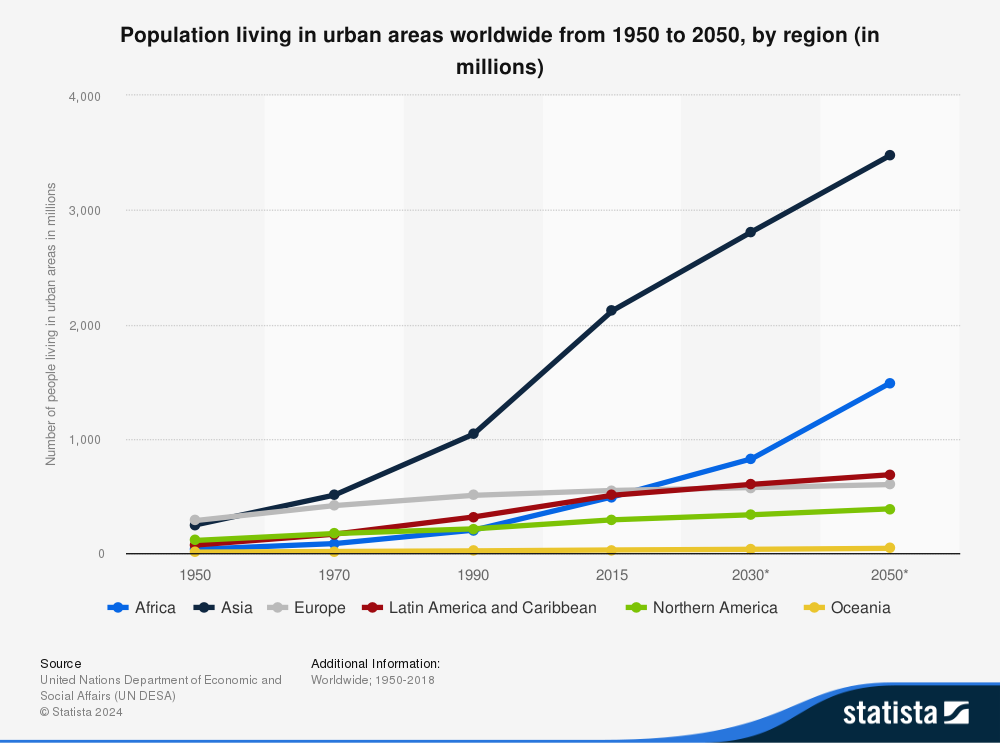
\includegraphics[scale=0.4]{statistic.png}
  \caption{Urbane Bevölkerung weltweit von 1950 bis 2050 nach Regionrafik~\cite{noauthor_change_nodate}}
  \label{statistic}
\end{figure}

Urbanisierungstrends sind je nach Region sehr unterschiedlich. 
In Ländern wie Europa und Nordamerika sind die Urbanisierungsraten bereits sehr hoch und liegen oft bei über 80 \%. 
Diese Regionen haben städtische Gebiete geschaffen und konzentrieren sich nun auf die Modernisierung der bestehenden Infrastruktur, um diese effizienter und nachhaltiger zu gestalten. 
Im Gegensatz dazu schreitet das Städtewachstum von  Entwicklungsländern wie Indien und Nigeria immer schneller an. 
Momentan liegt die Urbanisierungsrate bei etwa 35-40 \%, aber die Städte wachsen schnell, da die Landbevölkerung auf der Suche nach einer besseren Versorgung in städtische Zentren zieht. \autocite[S. 6ff]{taubenbock_globale_2015}
Ein weiterer auffälliger Aspekt der Urbanisierung ist die Zunahme von Megastädten, d. h. Städten mit mehr als 10 Millionen Einwohnern. 
Heute gibt es weltweit mehr als 30 Megastädte, darunter Tokio, Delhi und Shanghai, die als globale wirtschaftliche und kulturelle Zentren dienen. \autocite[S. 50]{taubenbock_globale_2015}
Die Urbanisierung ist jedoch nicht auf diese großen Städte beschränkt. 
Auch kleinere Städte mit weniger als einer Million Einwohnern erleben ein schnelles Wachstum. 
Diese Städte spielen eine entscheidende Rolle in der Stadtentwicklung und dienen oft als regionale Zentren für Innovation und wirtschaftliche Aktivitäten.

Neben Wirtschaftswachstum und technologischen Fortschritten bringt die Urbanisierung jedoch auch Herausforderungen mit sich. 
Die Städte müssen mit einer wachsenden Bevölkerung fertig werden, die angemessenen Wohnraum, Infrastruktur und öffentliche Dienstleistungen benötigt. 
Nachhaltige Stadtplanung und Investitionen in die Infrastruktur sind notwendig, um sicherzustellen, dass die Städte bei ihrem Wachstum lebenswert und integrativ bleiben. \autocite[S. 13ff]{zhang_trends_2015}
Dieses Gleichgewicht zwischen Wachstum und Nachhaltigkeit wird in den kommenden Jahrzehnten ein entscheidender Aspekt der Urbanisierung sein. 

\subsubsection{Urbanisierung als globaler Trend}
Die Urbanisierung verändert die Gesellschaften weltweit und beeinflusst die Art und Weise, wie Menschen leben, arbeiten und miteinander umgehen. 
Während Industrie- und Entwicklungsländer diesen Trend unterschiedlich erleben, stehen beide vor einer Mischung aus Herausforderungen und Chancen. 
Diese Komplexität erfordert einen genaueren Blick, nicht nur auf die Zahlen, sondern auch auf die einzigartigen Probleme und potenziellen Lösungen, mit denen Städte in aller Welt konfrontiert sind.

Das Wachstum der Städte hat sich im letzten Jahrhundert erheblich beschleunigt. 
In Industrieländern wie Deutschland, Japan und Kanada liegt die Urbanisierungsrate bei über 80 \%. 
In diesen Ländern liegt der Schwerpunkt auf der Erhaltung und Verbesserung der städtischen Infrastruktur, um mit dem technischen Fortschritt und den Umweltstandards Schritt zu halten. \autocite[S. 6ff]{taubenbock_globale_2015}
Kopenhagen zum Beispiel ist führend in der nachhaltigen Stadtplanung und verbindet erneuerbare Energiesysteme mit einem effizienten öffentlichen Nahverkehr. 
Umgekehrt erleben Städte in Entwicklungsregionen wie Afrika (besonders Städte südlich der Sahara) und Südasien explosionsartiges Wachstum. 

Lagos, Nigeria, ist beispielsweise eine der am schnellsten wachsenden Städte der Welt mit einer Bevölkerung, die sich seit 1990 fast vervierfacht hat. \autocite{aliyu_urbanization_2017}
Diese Länder stehen oft vor der doppelten Herausforderung, neue städtische Infrastrukturen zu bauen und gleichzeitig bestehende Mängel zu bewältigen. 
Die rasche Verstädterung in solchen Gebieten wird durch die Landflucht und wirtschaftliche Möglichkeiten angetrieben, kann aber auch zu informellen Siedlungen und überlasteten öffentlichen Diensten führen.


\subsubsection{Herausforderungen der Urbanisierung}
Urbanisierung stellt die Städte oft vor große Herausforderungen, die bewältigt werden müssen, um ein nachhaltiges und gerechtes Wachstum zu gewährleisten. 
Diese Herausforderungen reichen von der Infrastruktur über Umweltbelastungen bis hin zu sozialen Ungleichheiten und stellen Stadtplaner vor einzigartige Hindernisse.
Eines der dringendsten Probleme ist die unzureichende Infrastruktur. 
Während die Bevölkerung wächst, haben die Städte Schwierigkeiten, mit der Nachfrage nach grundlegenden Dienstleistungen wie Wohnraum, Transport und Abwasserentsorgung mitzuhalten. \autocite[S. 13ff]{zhang_trends_2015}
In Mumbai beispielsweise hat der Mangel an erschwinglichem Wohnraum zur Ausbreitung selbst errichteten Siedlungen geführt, in denen Millionen von Menschen ohne Zugang zu sauberem Wasser oder einem angemessenen Abwassersystem leben. \autocite{bhattarai_exposing_2020}
Dieser Mangel an Infrastruktur beeinträchtigt nicht nur die Lebensqualität, sondern schränkt auch das wirtschaftliche Potenzial ein und verschärft die Gesundheitsrisiken.
Der Druck auf die Umwelt nimmt ebenfalls zu, da städtische Gebiete für über 70 \% der weltweiten Kohlenstoffemissionen verantwortlich sind, was größtenteils auf den Verkehr, die Industrie und die Energienutzung zurückzuführen ist. \autocite[S. 192f]{taubenbock_globale_2015}
Die Auswirkungen auf die Umwelt sind in Städten wie Peking, wo die Luftverschmutzung durch Fahrzeuge und Fabriken ein ernsthaftes Risiko für die öffentliche Gesundheit darstellt, besonders deutlich zu spüren. \autocite{hao_improving_2005}
Küstenstädte wie Jakarta sind durch den Klimawandel zusätzlich bedroht, unter anderem durch den steigenden Meeresspiegel und vermehrte Überschwemmungen. 
Diese Umweltbelastungen erfordern innovative und kooperative Ansätze für die Stadtplanung und Nachhaltigkeitsinitiativen. \autocite{owen-burge_jakarta_2022}
Soziale Ungleichheit ist ein weiteres kritisches Thema, das durch die Urbanisierung verschärft wird. 
Die rasche Ausdehnung der Städte führt oft zu einer starken Kluft zwischen wohlhabenden und benachteiligten Vierteln. 
Städte wie Kapstadt in Südafrika veranschaulichen, wie historische Ungleichheiten im städtischen Umfeld noch verstärkt werden, da viele Bewohner informeller Siedlungen keinen Zugang zu Bildung, Gesundheitsversorgung und Beschäftigungsmöglichkeiten haben. 
Zersiedelung und Gentrifizierung vertiefen diese Gräben weiter, verdrängen einkommensschwache Gemeinschaften und schaffen Ausgrenzung-gebiete in zunehmend modernisierten städtischen Umgebungen. \autocite{turok_social_2021}

Um diese Herausforderungen zu bewältigen, brauchen die Städte umfassende und integrative Strategien, die dem gerechten Zugang zu Ressourcen, innovativen Infrastrukturlösungen und nachhaltigen Umweltpraktiken Vorrang einräumen. 
Ohne solche Maßnahmen könnten die mit einer ungebremsten Urbanisierung verbundenen Risiken ihre potenziellen Vorteile überwiegen, insbesondere für schwache Bevölkerungsgruppen.


\subsubsection{Chancen der Urbanisierung}
Trotz dieser Herausforderungen ermöglicht die Urbanisierung den gesellschaftlichen und wirtschaftlichen Fortschritt, insbesondere wenn sie mit einer effektiven Planung einhergeht. 
Städte haben als Zentren der Innovation und Konnektivität das Potenzial, globale Herausforderungen zu bewältigen und nachhaltiges Wachstum zu schaffen. \autocite[S. 5ff]{zhang_trends_2015}
Städte fördern technologische und soziale Innovationen, da sie Talente, Infrastrukturen und Ressourcen bündeln und damit ideale Zentren für die Entwicklung und Umsetzung von Lösungen sind. \autocite[S. 5ff]{zhang_trends_2015}
So können beispielsweise Smart-City-Technologien die Effizienz und Lebensqualität verbessern. 
Durch die Integration von \ac{IoT} und Big-Data-Analysen können Städte den Verkehrsfluss optimieren, den Energieverbrauch senken und die Abfallwirtschaft verbessern. 

Wirtschaftlich gesehen fungieren die städtischen Zentren als Wachstumsmotoren. 
Sie konzentrieren Unternehmen, fördern den Unternehmergeist und ziehen Investitionen an. 
Ein gut verwaltetes städtisches Umfeld kann wirtschaftliche Diversifizierung und Innovation weiter fördern. \autocite[S. 5ff]{zhang_trends_2015}
Städte wie Nairobi in Kenia entwickeln sich beispielsweise zunehmend zu regionalen Technologie- und Finanzzentren, die Arbeitsplätze schaffen und neue Branchen fördern. 
Diese Entwicklungen kommen nicht nur den Städten selbst zugute, sondern tragen durch die Förderung von Produktivität und Innovation auch erheblich zur nationalen Wirtschaft bei. \autocite{okland_nairobis_2019}
Die städtische Dichte kann, wenn sie richtig gesteuert wird, auch ein nachhaltigeres Leben ermöglichen. 
Die Bevölkerungskonzentration erleichtert die Einführung öffentlicher Nahverkehrssysteme, die Verringerung der Energieverschwendung und die Schaffung von Grünflächen. 
Beispiele wie die Fahrradinfrastruktur in Amsterdam zeigen, wie die Stadtgestaltung die Abhängigkeit vom Auto und die Kohlenstoffemissionen verringern kann. \autocite{buehler_cycling_2010}
Letztlich sind die Chancen, die die Urbanisierung bietet, beträchtlich, aber sie hängen von einer sorgfältigen Planung und Steuerung ab. 
Städte, die Inklusivität, Nachhaltigkeit und Innovation in den Vordergrund stellen, können die Urbanisierung als Kraft für einen positiven Wandel nutzen, das Wirtschaftswachstum ankurbeln, die Lebensqualität verbessern und zu globalen Lösungen für drängende Herausforderungen wie den Klimawandel und soziale Ungleichheit beitragen.

\subsection{Wie hängen Urbanisierung und digitale Transformation zusammen?}
Die Wechselwirkung zwischen Urbanisierung und digitaler Transformation
Urbanisierung und digitaler Wandel sind eng miteinander verwoben und beeinflussen und beschleunigen sich gegenseitig auf tiefgreifende Weise. 
Städte als Zentren der Bevölkerung und der Wirtschaftstätigkeit stehen vor Herausforderungen, die technologische Lösungen erfordern. 
Gleichzeitig verändert die Einführung digitaler Technologien die Art und Weise, wie Städte funktionieren und wachsen, und bietet neue Möglichkeiten für Nachhaltigkeit, Integration und Innovation. \autocite{european_commission_digital_2019}

Das rasante Wachstum der Städte erhöht den Bedarf an innovativen Werkzeugen zur Bewältigung städtischer Herausforderungen wie Überbevölkerung, Umweltbelastung und Infrastrukturanforderungen. 
Städte werden zum fruchtbaren Boden für die Erprobung und Einführung von Technologien, die diese Probleme wirksam angehen. 
Singapur ist ein Beispiel dafür, wie urbane Herausforderungen die digitale Innovation vorantreiben. 
Zu den dortigen Smart-City-Initiativen gehören \ac{KI}-gestützte Systeme zur Bewältigung von Verkehrsstaus, z. B. 
ein vorausschauendes Verkehrsmanagement, und \ac{IoT}-gestützte Technologien zur Wassereinsparung, die den Wasserverbrauch in der gesamten Stadt überwachen und optimieren. 
Diese Lösungen verbessern nicht nur die Effizienz, sondern auch die Qualität des städtischen Lebens. \autocite{noauthor_smart_nodate}
Dubai geht mit seinen ehrgeizigen Smart-City-Programmen noch einen Schritt weiter, indem es Blockchain für sichere Behördentransaktionen und \ac{KI} für die Optimierung der Ressourcennutzung einsetzt. 
Die Stadt hat die „Dubai Paperless Strategy“ umgesetzt, mit der Verwaltungsprozesse digitalisiert werden, um jährlich Millionen von Blatt Papier einzusparen, und gibt damit ein Beispiel dafür, wie digitale Lösungen die städtische Verwaltung verändern können. \autocite{noauthor_dubai_nodate}

Digitale Technologien haben auch Einfluss darauf, wie sich Städte entwickeln. 
Smart-City-Projekte veranschaulichen das transformative Potenzial von \ac{IoT}, \ac{KI} und Datenanalyse bei der Gestaltung nachhaltiger und integrativer städtischer Umgebungen. 
Amsterdam ist ein bemerkenswertes Beispiel, das mit seiner fahrradfreundlichen Infrastruktur zeigt, wie Technologie und Planung positive Auswirkungen haben können. 
Durch die Priorisierung der Fahrradinfrastruktur und den Einsatz von Datenanalysen bei der Planung von Radwegen reduziert Amsterdam Verkehrsstaus, senkt den Kohlendioxidausstoß und fördert einen gesünderen Lebensstil. 
Dieser Ansatz hat die Stadt zu einem der nachhaltigsten urbanen Zentren der Welt gemacht und zeigt, wie eine durchdachte Integration von Technologie ökologische und soziale Herausforderungen angehen kann. \autocite{buehler_cycling_2010}
Darüber hinaus fördern E-Governance-Plattformen eine größere Transparenz und bürgerschaftliches Engagement. 
Digitale Tools rationalisieren Dienstleistungen wie den öffentlichen Nahverkehr, die Versorgungsbetriebe und die Abfallentsorgung und sorgen für Zugänglichkeit und Effizienz für alle Einwohner. 
Diese Plattformen ermöglichen es den Stadtverwaltungen, sich schnell an die Bedürfnisse der Einwohner anzupassen, was die allgemeine Zufriedenheit und die Beteiligung am städtischen Leben verbessert.

Urbanisierung und digitale Transformation gehen Hand in Hand, um die Zukunft der Städte zu gestalten. 
Wachsende urbane Gebiete treiben die Nachfrage nach innovativen Technologien voran, und die fortschreitende digitale Transformation eröffnet neue Wege, um Städte nachhaltiger, inklusiver und effizienter zu machen. 
Städte wie Singapur, Dubai und Amsterdam zeigen, dass dieses Zusammenspiel nicht nur theoretisch ist, sondern bereits heute das städtische Leben verändert. 
Indem sie diese Synergie nutzen, können Städte Herausforderungen meistern, Chancen maximieren und eine Vorreiterrolle beim globalen Fortschritt übernehmen.


% Wechselwirkungen zwischen Urbanisierung und digitaler Transformation
% -------------------------------------------------------
\section{Wechselwirkungen zwischen Urbanisierung und digitaler Transformation}
\subsection{Urbane Herausforderungen, die durch digitale Transformation bewältigt werden können}
\subsubsection{Verkehr und Mobilität}
Mit dem Wachstum städtischer Gebiete wird die Verkehrsinfrastruktur zunehmend an ihre Belastungsgrenze gebracht. 
Probleme wie überfüllte Straßen, unzureichende öffentliche Verkehrssysteme und die steigende Zahl an privaten Fahrzeugen verursachen regelmäßige Staus, die zu erheblichen wirtschaftlichen Verlusten und einer Beeinträchtigung der Lebensqualität führen.
Umweltprobleme wie CO2-Emissionen, Lärmbelastung und Luftverschmutzung werden durch die Abhängigkeit von fossilen Brennstoffen weiter verschärft.
In vielen Städten fehlt es an nachhaltigen Alternativen wie einem gut ausgebauten Netz an Fahrradwegen, elektrischen Bussen oder Straßenbahnen. 
Ohne den Einsatz intelligenter Verkehrssysteme, die auf Technologien wie \ac{IoT} und Big Data basieren, wird es schwierig sein, die Mobilität effizient und nachhaltig zu gestalten. \autocite{mckinsey_global_institute_smart_2021}


\subsubsection{Wohnraum und Urbanisierung}
Der schnelle Anstieg von Menschen in urbane Zentren erhöht natürlich die Nachfrage nach Wohnraum und verschärft somit die Wohnungsnot. 
Besonders in wirtschaftlich aufstrebenden Städten führt dies zur Entstehung von informellen Siedlungen und Slums.
Diese Gebiete sind oft durch schlechte Lebensbedingungen geprägt, darunter fehlende Wasserversorgung, mangelhafte Entsorgungssysteme und fehlender Zugang zu Strom.
Parallel dazu steigen die Miet- und Kaufpreise in den zentralen Stadtteilen, was die Gentrifizierung fördert und einkommensschwache Gruppen an den Stadtrand drängt.
Ineffiziente Stadtplanung und der Druck, gleichzeitig Wohnraum zu schaffen und Umweltstandards einzuhalten, verschärfen die Herausforderung zusätzlich. \autocite{un_habitat_world_2022}


\subsubsection{Umwelt- und Ressourcenprobleme}
Die Urbanisierung bringt eine Vielzahl von Umweltbelastungen mit sich. 
Industrielle Emissionen, Verkehrsabgase und ein unzureichendes Abfallmanagement verschlechtern die Luft- und Wasserqualität. 
Auch die steigende Nachfrage nach Energie und Ressourcen führt zu einem erhöhten Druck auf fossile Brennstoffe, wodurch sich die globale Erwärmung beschleunigt.
Phänomene wie die Urban Heat Islands, bei denen sich Städte aufgrund der dichten Bebauung und fehlender Grünflächen stärker aufheizen, beeinflussen nicht nur  das Mikroklima negativ, sondern gefährden  ebenfalls die Gesundheit der Bewohner.
Effektive Lösungen wie grüne Dächer, nachhaltige Energiequellen oder smarte Abfallsysteme werden immer dringlicher. \autocite{sensors_smart_2015}


\subsubsection{Soziale Ungleichheit}
Urbanisierung kann bereits bestehende soziale Ungleichheiten weiter verschlimmern.
Benachteiligte Bevölkerungsgruppen haben oft keinen gleichberechtigten Zugang zu grundlegenden Infrastrukturen wie Bildung, Gesundheitsversorgung und sicherem Wohnraum.
Die digitale Kluft verstärkt diese Probleme zusätzlich, da ärmere Haushalte oft von Technologien ausgeschlossen sind, die beispielsweise Zugang zu Online-Bildung oder Telemedizin ermöglichen.
Auch die Verdrängung von einkommensschwachen Gruppen aus zentralen Stadtteilen durch steigende Mietpreise und Gentrifizierung vertieft die Kluft zwischen sozialen Schichten. \autocite{digital_how_2024}


\subsubsection{Infrastrukturüberlastung}
Städte weltweit stehen vor der Herausforderung, ihre Infrastruktur den wachsenden Bevölkerungszahlen anzupassen. 
Die Nachfrage nach Wasser, Energie und Entsorgungssystemen übersteigt häufig die Kapazitäten bestehender Systeme. 
Veraltete Wasserversorgungsnetze oder überlastete Stromnetze führen zu Ineffizienzen und wiederholten Versorgungsausfällen. 
Besonders in Megastädten wie Mumbai oder Lagos zeigt sich, dass Infrastruktur, die ursprünglich für kleinere Bevölkerungsmengen ausgelegt war, den Bedürfnissen moderner Großstädte nicht mehr gerecht wird. \autocite{mckinsey_global_institute_smart_2021}.


\subsubsection{Gesundheit und Lebensqualität}
Die Luftverschmutzung, ein Ergebnis von Verkehr, Industrie und unzureichendem Abfallmanagement, stellt eine ernsthafte Gefahr für die Gesundheit der städtischen Bevölkerung dar. 
Atemwegserkrankungen und Herz-Kreislauf-Probleme nehmen in urbanen Räumen zu. 
Gleichzeitig erhöhen psychosoziale Belastungen wie Stress, Hektik und der Mangel an Ruhe- und Grünflächen das Risiko für psychische Erkrankungen. 
Die unzureichende Verfügbarkeit von Gesundheitsdiensten in dicht besiedelten Gebieten und der Druck, schnellere Lösungen für Gesundheitsprobleme zu finden, verschlechtern die Lebensqualität. \autocite{un_habitat_world_2022}


\subsubsection{Sicherheit und Überwachung}
Die wachsende Bevölkerungsdichte in Städten erhöht das Risiko von Kriminalität, sozialen Konflikten und Katastrophen. 
Viele urbane Gebiete sind nicht ausreichend auf Notfälle wie Naturkatastrophen, Pandemien oder Terroranschläge vorbereitet. 
Gleichzeitig steigt der Bedarf an effektiven Überwachungssystemen und Sicherheitsstrategien. 
Der Einsatz moderner Technologien wie Gesichtserkennung und Sensorik birgt jedoch auch ethische Herausforderungen, insbesondere im Hinblick auf Datenschutz und die Privatsphäre der Bürger. \autocite{mckinsey_global_institute_smart_2021}


\subsubsection{Schlussfolgerung}
Die Urbanisierung bringt tiefgreifende Herausforderungen mit sich, die sich auf Mobilität, Wohnraum, Umwelt, soziale Gerechtigkeit, Infrastruktur, Gesundheit und Sicherheit erstrecken. 
Nur durch innovative Ansätze, smarte Technologien und gezielte Investitionen in nachhaltige Stadtplanung können diese Probleme bewältigt werden. 
Ein stärkerer Fokus auf integrative und technologische Lösungen ist notwendig, um Städte zukunftsfähig und lebenswert zu gestalten.


\subsection{Warum Urbanisierung die digitale Transformation beschleunigt}

\subsubsection{Effizienz durch Smart Cities}
Urbanisierung setzt Städte unter Druck, moderne technologische Lösungen zu integrieren, um ihre Infrastrukturen an die steigenden Bevölkerungszahlen anzupassen.
Die Urbanisierung schafft ebenfalls eine ideale Umgebung für Smart-City-Initiativen. 
Städte nutzen digitale Technologien wie das \ac{IoT}, \ac{KI} und Big Data, um Infrastrukturen intelligenter und effizienter zu gestalten und um Ressourcen effizienter zu verwalten.
Ein Beispiel ist die Implementierung intelligenter Verkehrssysteme, die Verkehrsflüsse optimieren und Umweltbelastungen reduzieren. 
Solche Technologien sind nur durch den digitalen Fortschritt möglich, der durch die Urbanisierung stark vorangetrieben wird, da Städte zunehmend auf diese Lösungen angewiesen sind, um ihre Effizienz und Nachhaltigkeit zu gewährleisten.
Solche Technologien wären ohne die durch die Urbanisierung geschaffenen Herausforderungen und Bedürfnisse kaum entwickelt worden. \autocite{mckinsey_global_institute_smart_2021}


\subsubsection{Nachhaltigkeit durch Ressourcennutzung}
Städtische Ballungszentren, die für rund 70 Prozent des globalen Energieverbrauchs verantwortlich sind, profitieren stark von der digitalen Transformation. 
Intelligente Stromnetze (Smart Grids) und \ac{IoT}-gestützte Energieüberwachungssysteme helfen Städten, den Energieverbrauch zu optimieren und erneuerbare Energien besser in das bestehende Netz zu integrieren.
Die Urbanisierung fordert somit die Entwicklung solcher Systeme, die ohne den Druck steigender Bevölkerungszahlen nicht in diesem Maße notwendig wären. \autocite{sensors_smart_2015}
 

\subsubsection{Veränderung von Wirtschaft und Arbeitswelt}
Die Urbanisierung schafft dichte Arbeits- und Wirtschaftszentren, die digitale Transformation beschleunigen, indem sie neue Geschäftsmodelle und Arbeitsweisen ermöglichen.
Digitale Plattformen und Technologien fördern die Remote-Arbeit und Co-Working-Spaces, was insbesondere in hoch urbanisierten Regionen zunehmend an Bedeutung gewinnt.
Auch im Bereich der Bildung und Weiterbildung bieten digitale Plattformen Möglichkeiten, um Menschen für die Anforderungen einer technologisierten Wirtschaft auszubilden. \autocite{digital_how_2024}


\subsubsection{Digitale Plattformen als Lösung für urbane Bedürfnisse}
Die Urbanisierung hat die Nachfrage nach digitalen Dienstleistungen und Plattformen wie Lieferdiensten, Ridesharing und Online-Marktplätzen erhöht. 
Unternehmen wie Uber, Amazon und Airbnb haben ihre Geschäftsmodelle gezielt auf urbane Märkte abgestimmt, da die hohe Bevölkerungsdichte in Städten ideale Bedingungen für die Skalierung dieser Dienste bietet. 
Diese Plattformen basieren auf digitalen Technologien und haben ihre Entwicklung durch die städtische Nachfrage beschleunigt.\autocite{sustainability_digital_2023}


\subsubsection{Veränderung von Arbeits- und Wirtschaftsmustern}
Die Urbanisierung spielt eine zentrale Rolle bei der Beschleunigung der digitalen Transformation, indem sie dichte Arbeits- und Wirtschaftszentren schafft, die neue Geschäftsmodelle und Arbeitsweisen fördern. 
In stark urbanisierten Regionen werden digitale Lösungen zunehmend notwendig und bedeutend, um den wachsenden Anforderungen der städtischen Lebensweise gerecht zu werden. 
So entstehen zum Beispiel in großen Städten digitale Plattformen wie Slack und Zoom, die hybride Arbeitsmodelle und Remote Work ermöglichen. 
Diese Technologien steigern nicht nur die Flexibilität, sondern auch die Produktivität der Arbeitskräfte, da sie ortsunabhängiges Arbeiten und eine schnelle Kommunikation auch über große Distanzen hinweg erlauben.
Die enge Vernetzung und hohe Dichte von Menschen und Unternehmen in urbanen Zentren fördern das Entstehen dynamischer Arbeitsmärkte, in denen digitale Innovationen besonders schnell angenommen werden. 
Besonders deutlich wird dies bei der Zunahme von Co-Working-Spaces, die in vielen Städten als Antwort auf den begrenzten physischen Raum und die Nachfrage nach flexiblen Arbeitsplätzen entstanden sind. 
Diese Trends zeigen, dass die Urbanisierung eine treibende Kraft für die digitale Transformation ist, da sie die Notwendigkeit und Akzeptanz für digitale Technologien in der Arbeitswelt fördert.
Die Corona-Pandemie hat diesen Trend noch verstärkt, da der Bedarf nach digitalen Arbeitslösungen in urbanen Zentren, in denen physische Interaktionen durch Raumbegrenzungen und Gesundheitsvorkehrungen eingeschränkt waren, stark anstieg. 
Die Nutzung von digitalen Plattformen für Kommunikation und Zusammenarbeit wurde in dieser Zeit unverzichtbar und beschleunigte die Anpassung an digitale Arbeitsweisen. 
Urbanisierung hat somit nicht nur die Einführung neuer Technologien begünstigt, sondern auch die Entstehung von digitalen Arbeitsmodellen, die auch in Zukunft eine zentrale Rolle spielen werden. \autocite{sustainability_digital_2023}


\subsubsection{ Verbesserte städtische Dienstleistungen}
Mit der zunehmenden Urbanisierung steigt die Nachfrage nach effizienten städtischen Dienstleistungen wie Energieversorgung, Abfallwirtschaft und öffentlichem Verkehr. 
Digitale Technologien ermöglichen es Städten, diese effizienter und Bürger-zentrierter zu gestalten. 
E-Government-Plattformen wie sie in Estland entwickelt wurden, bieten Bürgern Zugang zu Verwaltungsdiensten über das Internet, was besonders in dicht besiedelten städtischen Gebieten Vorteile bringt. \autocite{un_habitat_world_2022}


\subsubsection{Bürger zentrierte Stadtplanung}
Die Urbanisierung treibt auch neue Ansätze in der Stadtplanung voran. 
Virtuelle Simulationen und \ac{BIM} ermöglichen es Stadtplanern, städtische Entwicklungsprojekte zu modellieren und deren Auswirkungen zu analysieren. 
Dadurch können Städte proaktiv auf die Bedürfnisse ihrer Bewohner eingehen und Probleme wie Wohnungsnot oder Verkehrsüberlastung besser lösen. \autocite{mckinsey_global_institute_smart_2021}


\subsubsection{Datengetriebene Umweltpolitik}
Die Urbanisierung verstärkt Umweltprobleme wie Luftverschmutzung und Ressourcenknappheit, was Städte dazu zwingt, innovative technologische Lösungen einzusetzen. 
Sensornetzwerke, die beispielsweise die Luftqualität in Echtzeit überwachen, ermöglichen datenbasierte Entscheidungen, etwa zur Verkehrslenkung oder zur Reduktion von Emissionen. 
Zudem fördern Apps wie Ökotracker das Bewusstsein und die aktive Beteiligung der Bürger an nachhaltigem Handeln. 
Diese Technologien beschleunigen die digitale Transformation, indem sie die Nachfrage nach datenintensiven Systemen, Cloud-Diensten und \ac{IoT}-Infrastrukturen erhöhen. 
Die Urbanisierung schafft somit nicht nur die Probleme, sondern auch die Grundlage für die Entwicklung und Einführung solcher digitaler Innovationen. \autocite{sensors_smart_2015}

 
\subsubsection{Kreislaufwirtschaft und Abfallmanagement}
In dicht besiedelten urbanen Gebieten fällt besonders viel Abfall an, wodurch effiziente Systeme zur Ressourcenverwaltung notwendig werden. 
Städte wie Kopenhagen nutzen \ac{IoT}-Sensoren, um die Füllstände von Müllcontainern in Echtzeit zu überwachen und darauf basierend Abholrouten zu optimieren. 
Dies reduziert sowohl Kosten als auch den C02-Ausstoß der Entsorgungsfahrzeuge. 
Solche datengetriebenen Ansätze entstehen direkt aus der Dringlichkeit, urbane Herausforderungen effizient zu lösen, und treiben die digitale Transformation voran, indem sie die Integration von IoT und künstlicher Intelligenz in städtische Infrastrukturen fördern. 
Urbanisierung wird so zu einem Katalysator für technologische Innovationen im Bereich nachhaltiger Ressourcennutzung. \autocite{sensors_smart_2015}


\subsubsection{Schlussfolgerung}
Die Urbanisierung wirkt als Beschleuniger der digitalen Transformation, indem sie die Nachfrage nach technologischen Innovationen antreibt und Städte dazu zwingt, effizientere Lösungen für ihre wachsenden Herausforderungen zu entwickeln. 
Smart Cities, digitale Arbeitswelten, nachhaltige Infrastrukturen und datengetriebene Umweltpolitik sind nur einige Beispiele für die Synergie zwischen Urbanisierung und Digitalisierung. 
Während diese Transformation enorme Chancen bietet, ist es essenziell, dass sie inklusiv und nachhaltig gestaltet wird, um langfristig eine höhere Lebensqualität in urbanen Räumen zu gewährleisten.


\subsection{Wie digitale Transformation die Urbanisierung beschleunigt}
\subsubsection{Verkehr und Mobilität}
Die Einführung digitaler Technologien wie Echtzeit-Navigation, \ac{KI}-optimierter Verkehrssteuerung und Plattformen für geteilte Mobilität (z. B. Ridesharing) steigert die Effizienz und Bequemlichkeit des Transports in Städten. 
Diese Verbesserungen machen städtische Gebiete für Menschen attraktiver, da sie die Herausforderungen von Staus und ineffizientem Pendeln mindern. 
Dadurch ziehen mehr Menschen in Städte, da die Mobilität in urbanen Räumen einfacher und zuverlässiger wird. \autocite{mckinsey_global_institute_smart_2021}

\subsubsection{Wohnraum und Urbanisierung}
Fortschritte in der Stadtplanung durch digitale Tools wie \\ \ac{GIS} ermöglichen eine schnellere und effizientere Entwicklung urbaner Gebiete. 
Smarte Technologien in Wohngebäuden verbessern die Ressourcennutzung, was besonders in dicht besiedelten Städten von Vorteil ist. 
Die dadurch geschaffenen moderneren, nachhaltigeren Wohnmöglichkeiten fördern die Urbanisierung, da sie die Attraktivität städtischen Lebens erhöhen. \autocite{un_habitat_world_2022}

\subsubsection{Umwelt- und Ressourcenprobleme}
Smarte Technologien wie \ac{IoT}-Sensoren und \ac{KI}-basierte Energiemanagementsysteme machen Städte ressourceneffizienter und umweltfreundlicher. 
Das steigert die Lebensqualität und zieht Unternehmen sowie Menschen an, die von nachhaltigen Lebensbedingungen profitieren möchten. 
Der technologische Fortschritt reduziert Umweltprobleme und ermöglicht städtisches Wachstum mit weniger ökologischen Auswirkungen. \autocite{sensors_smart_2015}

\subsubsection{Soziale Ungleichheit}
Digitale Bildung und Telemedizin schaffen einen breiteren Zugang zu grundlegenden Dienstleistungen, was bisher benachteiligte Bevölkerungsgruppen in die Lage versetzt, in städtische Räume zu ziehen. 
Die digitale Transformation erhöht somit die Inklusion und macht Städte zu Zentren für wirtschaftliche und soziale Möglichkeiten, die mehr Menschen anziehen. \autocite{digital_how_2024}

\subsubsection{Infrastrukturüberlastung}
Technologien wie digitale Zwillinge (Digital Twins) und \ac{IoT} ermöglichen die effizientere Planung und Nutzung urbaner Infrastrukturen. 
Dies hilft Städten, den Anforderungen wachsender Bevölkerungszahlen gerecht zu werden, ohne dass die Lebensqualität leidet. 
Dadurch wird das Leben in Städten auch für zukünftige Generationen attraktiver, was die Urbanisierung beschleunigt. \autocite{mckinsey_global_institute_smart_2021}

\subsubsection{Gesundheit und Lebensqualität}
Fortschritte bei Gesundheitsapps, Wearables und intelligenten Umweltsensoren verbessern die Lebensqualität in städtischen Gebieten. 
Ein besseres Stadtklima und eine optimierte Gesundheitsversorgung locken mehr Menschen an, die eine hohe Lebensqualität und moderne medizinische Versorgung suchen. \autocite{un_habitat_world_2022}.

\subsubsection{Sicherheit und Überwachung}
Intelligente Sicherheits- und Überwachungssysteme sowie datenbasierte Notfallpläne erhöhen das Gefühl von Sicherheit in Städten. 
Dies fördert das Vertrauen von Menschen und Unternehmen in urbane Räume und verstärkt die Urbanisierung, da eine sichere Umgebung ein grundlegender Faktor für die Wahl des Lebensortes ist. \autocite{mckinsey_global_institute_smart_2021}


\subsubsection{Ergebnis}
Die Wechselwirkung zwischen Urbanisierung und digitaler Transformation ist ein kontinuierlicher und gegenseitiger Prozess.
Auf der einen Seite beschleunigt Urbanisierung die digitale Transformation, da die wachsende Bevölkerungsdichte in Städten die Nachfrage nach innovativen technologischen Lösungen steigert. 
Intelligente Verkehrssysteme, automatisierte Energiemanagementlösungen und \ac{IoT}-basierte Infrastrukturen entstehen, um den Herausforderungen überfüllter urbaner Räume gerecht zu werden. 
Solche Technologien optimieren die Ressourcennutzung und erhöhen die Effizienz städtischer Dienste, was die Entwicklung und Implementierung digitaler Innovationen fördert.
Auf der anderen Seite begünstigt die digitale Transformation die Urbanisierung. 
Fortschritte in digitalen Technologien wie 5G-Netzwerken, Cloud-Computing und flexiblen Arbeitsmodellen erlauben es, urbane Lebensweisen besser zu unterstützen. 
Menschen können durch diese Technologien effektiver vernetzt arbeiten und die Vorteile städtischer Infrastruktur nutzen, ohne physisch an einen Arbeitsplatz gebunden zu sein. 
Diese Möglichkeiten machen das urbane Leben attraktiver, was den Zuzug in Städte und die damit verbundene Nachfrage nach Wohnraum und Infrastruktur zusätzlich antreibt.
So entwickeln sich Urbanisierung und digitale Transformation durch ihre gegenseitige Beeinflussung dynamisch weiter. 


\subsection{Grenzen, Risiken und ethische Aspekte der digitalen Stadtentwicklung}
Die digitale Stadtentwicklung bietet zahlreiche Chancen zur Verbesserung der Lebensqualität, Effizienz und Nachhaltigkeit in urbanen Zentren. 
Gleichzeitig gibt es bedeutsame Grenzen, Risiken und ethische Herausforderungen, die berücksichtigt werden müssen. 
Im Folgenden werden wichtige Aspekte beleuchtet, wobei besondere Rücksicht auf bestehende Studien und Berichte genommen wird.

\subsubsection{Grenzen der digitalen Stadtentwicklung}
Technologische Grenzen bestehen, da trotz stetiger Weiterentwicklung der digitalen Technologien weiterhin technische Hürden und Einschränkungen vorhanden sind. 
Beispielsweise sind bestehende Infrastrukturen oft nicht mit modernen digitalen Lösungen kompatibel, was wiederum zu hohen Umbaukosten und komplexen Integrationsprozessen führen kann. \autocite{kitchin_ethics_2016} 
Auch stellen die Anforderungen an Datenspeicherung und -verarbeitung eine Herausforderung dar, da städtische Infrastrukturen regelmäßig große Mengen an Daten generieren.

Finanzielle und politische Limitierungen zeigen sich, weil die Finanzierung großer Digitalisierungsprojekte in Städten häufig eine Herausforderung darstellt. 
Budgetbeschränkungen und der wirtschaftliche Druck auf öffentliche Haushalte können dazu führen, dass notwendige Investitionen in digitale Infrastrukturen nicht in ausreichendem Maße getätigt werden. \autocite{hamilton_funding_2017} 
Zudem sind politische Hürden und langsame Entscheidungsprozesse oft Hindernisse für eine zügige Implementierung digitaler Stadtentwicklung.

\subsubsection{Risiken der digitalen Stadtentwicklung}
Bei der zunehmenden Vernetzung von städtischen Systemen steigt das Risiko von Cyberangriffen und Datenmissbrauch, da kritische Infrastrukturen wie Energie- und Wasserversorgung besonders anfällig für Angriffe sind, die erhebliche Auswirkungen auf die öffentliche Sicherheit haben könnten. \autocite{anwar_smart_2022}

Auch werfen die Verwendung von Technologien wie Gesichtserkennung und Sensornetzwerken in städtischen Umgebungen gravierende Datenschutz- und Überwachungsfragen auf. 
Der Umgang mit personenbezogenen Daten muss sorgfältig geregelt werden, um die Privatsphäre zu schützen und den Missbrauch von Daten zu verhindern \autocite{hongladarom_shoshana_2023}.

\subsubsection{Ethische Aspekte der digitalen Stadtentwicklung}
Soziale Ungleichheit könnte verstärkt werden, da digitale Technologien bestehende soziale Ungleichheiten potenziell verschärfen. 
Ungleicher Zugang zu digitalen Dienstleistungen und Technologien kann eine digitale Kluft zwischen verschiedenen Bevölkerungsgruppen erzeugen \autocite{helsper_corresponding_2012}.

Inklusion und Partizipation sind wesentliche Aspekte einer nachhaltigen Stadtentwicklung. 
Es ist entscheidend, dass alle relevanten Interessengruppen einbezogen werden, insbesondere marginalisierte Gemeinschaften, um integrative Lösungen zu schaffen \autocite{arnstein_ladder_1969}. 
Digitale Plattformen spielen dabei eine wichtige Rolle, um die Partizipation zu fördern, erfordern jedoch eine gezielte Strategie zur Gewährleistung tatsächlich partizipativer Prozesse.

Zusammenfassend bietet die digitale Stadtentwicklung vielfältige Möglichkeiten zur Verbesserung der Lebensqualität in urbanen Räumen, geht jedoch mit signifikanten Herausforderungen einher. 
Es ist wichtig, technologische und finanzielle Grenzen sowie Sicherheitsrisiken sorgfältig anzugehen. 
Datenschutz- und ethische Aspekte dürfen nicht vernachlässigt werden, um sicherzustellen, dass die digitale Transformation inklusiv und gerecht erfolgt. 
Zukünftige Entwicklungen sollten durch umfassende Strategien begleitet werden, die Risiken minimieren und den Nutzen für alle Bürger maximieren.


% Digitale Transformation als Lösung für urbane Herausforderungen
% -------------------------------------------------------
\section{Digitale Transformation als Lösung für urbane Herausforderungen}
Digitale Technologien eröffnen zahlreiche Möglichkeiten zur Bewältigung der Herausforderungen der Urbanisierung. 
Durch praxisnahe Beispiele und Fallstudien wird veranschaulicht, wie Städte bereits erfolgreich digitale Ansätze integriert haben. 
Zusätzlich werden Zukunftsperspektiven skizziert, um eine Vision von modernen, nachhaltigen Städten der Zukunft zu entwickeln

\subsection{Fallstudien und Praxisbeispiele}
Der Bereich Mobilität und Verkehr wird oft durch das Beispiel Singapur illustriert, das als Vorreiter in der Anwendung intelligenter Verkehrssysteme gilt. 
Die Stadt nutzt ein umfassendes Verkehrsmanagementsystem, das auf Echtzeit-Daten von Sensoren und Kameras basiert, um den Verkehrsfluss zu optimieren und Staus zu minimieren \autocite{Chin2020}. 
Zudem fördert Singapur die Nutzung öffentlicher Verkehrsmittel und Car-Sharing-Modelle, unterstützt durch digitale Plattformen, um den individuellen Autoverkehr zu verringern.

Im Bereich nachhaltige Energie hat Amsterdam das "City of Amsterdam Smart City" -Projekt ins Leben gerufen, das darauf abzielt, die Energieeffizienz zu steigern und Emissionen zu reduzieren. 
Durch den Einsatz von intelligenten Zählern und erneuerbaren Energien wird die Energieverteilung optimiert. 
\ac{IoT}-Technologie ermöglicht die Überwachung von Verbrauchsmustern, um die Energieversorgung bedarfsgerecht anzupassen \autocite{Amsterdam2021}.

Toronto hat sich im digitalen Gesundheitswesen hervorgetan, indem es ein Pilotprojekt zur Telemedizin gestartet hat, das es Bürgern ermöglicht, auf medizinische Dienstleistungen zuzugreifen, ohne physisch in Arztpraxen präsent sein zu müssen. 
Dies reduziert die Belastung städtischer Kliniken und verbessert den Zugang zu Gesundheitsdiensten, insbesondere für Senioren und Menschen mit eingeschränkter Mobilität \autocite{Doe2022}.

In San Francisco wurde ein fortschrittliches Abfallmanagementsystem implementiert, das auf digitalen Technologien basiert. 
Mithilfe von \ac{IoT}-basierten Sensoren wird der Füllstand von Müllcontainern überwacht, um Abholrouten effizient zu planen und den CO2-Ausstoß zu verringern \autocite{Jones2019}. 
Dieses System hat dazu beigetragen, die Recyclingraten erheblich zu steigern und die Deponielasten zu reduzieren.

\subsection{Zukunftsperspektiven: Die Stadt der Zukunft}
Das Konzept der vernetzten Stadt wird in der Zukunft eine Schlüsselrolle spielen. 
Technologien wie 5G, \ac{IoT} und Cloud-Computing werden vollständig integrierte städtische Ökosysteme schaffen, in denen alle Infrastrukturen miteinander kommunizieren, um sowohl Ressourcen als auch Sicherheitsmaßnahmen effizient zu steuern.

Künstliche Intelligenz wird zunehmend in der Stadtplanung eingesetzt werden, um datengetriebene Erkenntnisse zu gewinnen und die Lebensqualität zu verbessern. 
Anwendungsbeispiele umfassen optimierte Verkehrssteuerung, effizientere öffentliche Dienstleistungen und intelligente Energienetze.

Zukünftige Städte werden Technologien nutzen, um nachhaltige Praktiken zu fördern und widerstandsfähige Systeme gegen den Klimawandel zu entwickeln. 
Dies umfasst die Integration von grüner Infrastruktur, erneuerbaren Energiequellen und nachhaltigen Gebäudetechnologien.

Die Einbindung der Bürger in die Entwicklung intelligenter Städte wird essenziell sein. 
Plattformen für Bürgerbeteiligung und Co-Creation ermöglichen den Einwohnern die aktive Mitgestaltung ihrer städtischen Umgebung, wodurch ihre Bedürfnisse und Wünsche besser adressiert werden.

Zusammenfassend stellt die digitale Transformation einen essenziellen Baustein für die Bewältigung urbaner Herausforderungen dar. 
Fallstudien zeigen, dass viele Städte weltweit bereits innovative digitale Lösungen implementiert haben, um ihre Effizienz, Nachhaltigkeit und Lebensqualität zu steigern. 
Angesichts der urbanen Zukunft ist es unabdingbar, dass Städte weiterhin in digitale Innovationen investieren und gleichzeitig eine inklusive und nachhaltige Entwicklung sicherstellen. 
Die Stadt der Zukunft wird nicht nur technologisch fortschrittlich, sondern auch lebenswert und anpassungsfähig sein.


% --------------------------------------------------------------------
\section*{Abkürzungen}
\addcontentsline{toc}{section}{Abkürzungen}

% Abkürzungsverzeichnis
\begin{acronym}[BIM]
  \acro{BIM}{Building Information Modeling}  
  \acro{dT}{digitale Transformation}  
  \acro{GIS}{Geoinformationssysteme}  
  \acro{IoT}{Internet of Things}  
  \acro{KI}{künstliche Intelligenz}  
  \acro{UN}{United Nations}  
\end{acronym}

% Literaturverzeichnis
\addcontentsline{toc}{section}{Literatur}
\printbibliography

\end{document}
